\documentclass[11pt]{article}

\usepackage[margin=1in]{geometry}
\usepackage{amsmath, amssymb}
\usepackage{booktabs}
\usepackage{graphicx}
\usepackage{siunitx}
\usepackage{hyperref}
\usepackage{xcolor}
\usepackage{listings}

\emergencystretch=2em

\lstset{
  language=Python,
  basicstyle=\small\ttfamily,
  keywordstyle=\bfseries,
  commentstyle=\itshape\color{gray},
  showstringspaces=false,
  breaklines=true,
  columns=fullflexible,
  frame=single,
  framesep=4pt,
  xleftmargin=4pt,
  xrightmargin=4pt,
}

\title{Independent Cross-Check of the GRAPE Optimizer\\
\large QuTiP \texttt{sesolve} vs.\ the Optimizer's Own Propagator}
\author{}
\date{}

\begin{document}
\sloppy
\maketitle

\section{Motivation}
\label{sec:motivation}

The GRAPE optimizer in this project designs microwave pulses and then reports how good those
pulses are, using the same block of code both times. That is worth worrying about. If the code
that grades a pulse had a mistake in it, the optimizer would still converge, and the reported
fidelity would still look good, just wrong. There would be no warning sign from inside the code
itself, since the optimizer, its gradient, and its own fidelity report all come from the same
source.

To catch a mistake like that, the pulses need to be checked with a second, separate tool that was
not built from the same code. This report uses QuTiP, a well established, independently written
quantum simulation library, to replay every saved pulse and recompute its fidelity from scratch.
If QuTiP's answer matches the optimizer's own answer, that is real evidence the waveforms do what
they are reported to do, not just that the code agrees with itself.

\section{Why the Cross-Check Is Actually Independent}
\label{sec:independence}

An agreement check only proves something if the two things being compared do not secretly rely on
the same code. If they did, a mistake in that shared code would show up identically on both sides,
and the check would pass even though the result is wrong. The comparison used here is independent
in two separate ways: the physical setup is built twice from scratch in two unrelated coding
styles, and the two sides use two completely different methods to simulate time evolution.

\subsection{The Hamiltonian Is Built Twice}

One version is plain NumPy. The operators are built as matrices by hand and combined with the
Kronecker product:

\begin{lstlisting}
a = np.diag(np.sqrt(np.arange(1, n_c)), 1)   # cavity lowering operator
b = np.diag(np.sqrt(np.arange(1, n_t)), 1)   # transmon lowering operator
A = np.kron(np.eye(n_t), a)                  # cavity operator, joint space
B = np.kron(b, np.eye(n_c))                  # transmon operator, joint space

H0 = chi * (A.conj().T @ A) @ (B.conj().T @ B) + ...
Hc = [A + A.conj().T, 1j*(A - A.conj().T), B + B.conj().T, 1j*(B - B.conj().T)]
\end{lstlisting}

The other version is built entirely from QuTiP's own operator objects, with no matrix written by
hand:

\begin{lstlisting}
a = qt.destroy(n_c)
b = qt.destroy(n_t)
A = qt.tensor(qt.qeye(n_t), a)
B = qt.tensor(b, qt.qeye(n_c))

H0 = chi * (A.dag()*A) * (B.dag()*B) + ...
Hc = [A + A.dag(), 1j*(A - A.dag()), B + B.dag(), 1j*(B - B.dag())]
\end{lstlisting}

Both blocks of code describe the same physical system: the dispersive coupling, and the cavity
and transmon anharmonicity. But they share no code path. A mistake in how one builds its operators
would not automatically appear in the other.

\subsection{The Propagator Is Built Twice}

One approach treats each time step as constant and finds the exact evolution by diagonalizing the
Hamiltonian directly:

\begin{lstlisting}
Hk = H0 + u[0]*Hc[0] + u[1]*Hc[1] + u[2]*Hc[2] + u[3]*Hc[3]
w, V = eigh(Hk)
Uk = V @ np.diag(np.exp(-1j * dt * w)) @ V.conj().T
\end{lstlisting}

The other approach hands the same step function to an adaptive ODE solver, which integrates the
Schr\"odinger equation numerically instead of diagonalizing anything:

\begin{lstlisting}
H = qt.QobjEvo([H0, [Hc[0], coeff0], [Hc[1], coeff1], [Hc[2], coeff2], [Hc[3], coeff3]])
result = qt.sesolve(H, psi0, tlist)
\end{lstlisting}

These are not two implementations of the same algorithm. They are two different numerical methods
solving the same physics problem. A mistake specific to either one would show up as a
disagreement, not a silent match.

\subsection{What Is Actually Shared}

The only things the two sides genuinely share are the physical constants, the pulse being tested,
and the definition of a successful gate. That sharing is unavoidable and correct: the goal is to
ask two different methods the same physical question, not two different questions. Because the
two sides share only the physics and not the code, agreement between them is real evidence the
simulation is computing the right answer, not evidence that the code agrees with itself.

\subsection{Turning the Pulse Into a QuTiP Object}

One more detail is worth showing directly: how the raw pulse, a plain array of numbers, gets
handed to the ODE solver without being changed along the way.

The optimizer's pulse is piecewise constant. Each of the four control channels is held fixed for
one time step and then jumps to the next value. QuTiP needs that same pulse as a time-dependent
coefficient it can evaluate at any time the solver asks for. The setting \texttt{order=0} below
tells QuTiP to hold each value flat until the next time point, called zero-order hold, instead of
smoothly interpolating between points:

\begin{lstlisting}
coeff = qt.coefficient(u_column, tlist=tlist, order=0)   # zero-order hold
H = qt.QobjEvo([H0, [Hc0, coeff0], [Hc1, coeff1], [Hc2, coeff2], [Hc3, coeff3]])
result = qt.sesolve(H, psi0, tlist)
\end{lstlisting}

With \texttt{order=0}, the solver sees exactly the same step-function pulse the optimizer
produced. There is no smoothing, no interpolation, and no rounding. A mismatch between the two
fidelities cannot be blamed on QuTiP simulating a slightly different waveform, because it is
simulating the same one.

\section{Results}
\label{sec:results}

Every saved pulse was checked this way: the six single-qubit logical gates on the cat-code qubit
($X$, $Y$, $Z$, $H$, $T$, $I$), the encode and decode unitaries ($U_{\mathrm{enc}}$,
$U_{\mathrm{dec}}$), and the $|g,0\rangle \to |g,6\rangle$ Fock-state preparation pulse. For each
pulse, fidelity was computed with both methods at ten cavity truncations,
$n_c \in \{22, 24, 26, 28, 30, 32, 34, 36, 38, 40\}$, and the absolute difference
$|F_{\mathrm{grape\_core}} - F_{\mathrm{qutip}}|$ was recorded.

\begin{table}[h]
\centering
\begin{tabular}{lS[table-format=1.2e1]}
\toprule
{Pulse} & {Max $|\Delta F|$} \\
\midrule
$g0 \to g6$ prep & 6.28e-7 \\
$X$              & 1.99e-6 \\
$Y$              & 1.56e-6 \\
$Z$              & 2.62e-8 \\
$H$              & 3.47e-7 \\
$T$              & 5.26e-8 \\
$I$              & 2.62e-8 \\
$U_{\mathrm{enc}}$ & 1.07e-6 \\
$U_{\mathrm{dec}}$ & 8.90e-7 \\
\bottomrule
\end{tabular}
\caption{Maximum $|F_{\mathrm{grape\_core}} - F_{\mathrm{qutip}}|$ per pulse, over all ten cavity
truncations tested. All values sit at or below the working tolerance of an adaptive ODE solver
($\sim 10^{-6}$ relative), i.e.\ at the noise floor of the independent method itself rather than
at a level indicating disagreement.}
\label{tab:summary}
\end{table}

The worst case across all nine pulses and all ten truncations is $1.99\times10^{-6}$ ($X$ gate).
Every other pulse agrees to within $10^{-6}$ or better. Figure~\ref{fig:validation} shows the full
per-truncation breakdown for each pulse.

\begin{figure}[h]
\centering
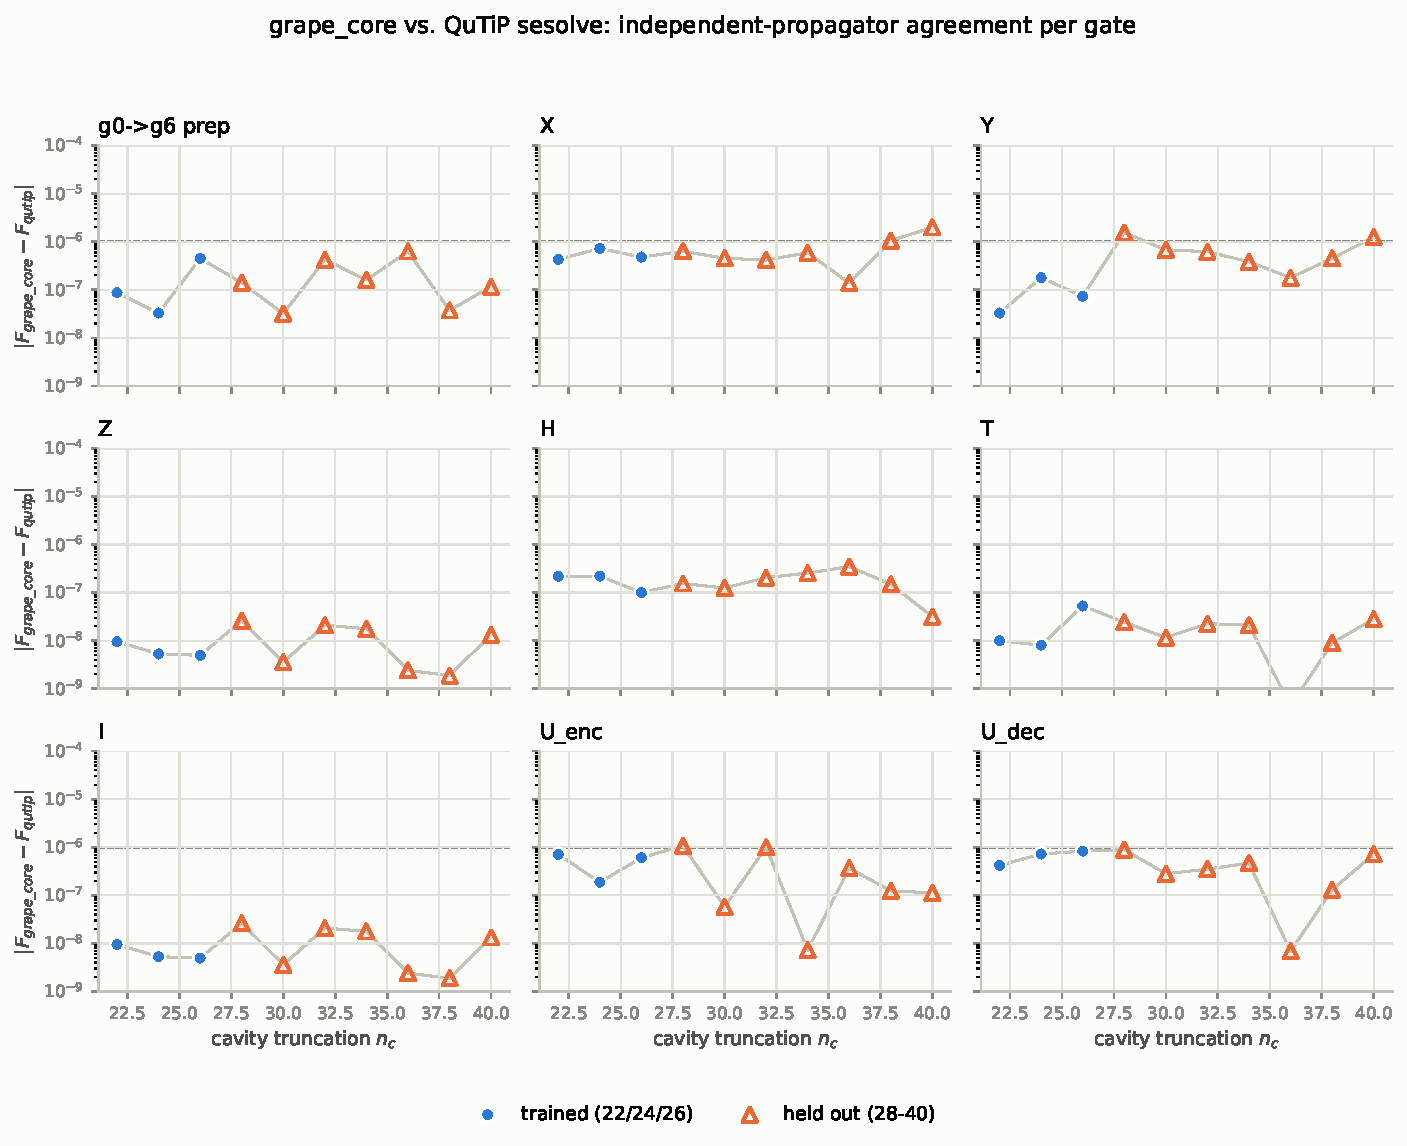
\includegraphics[width=0.95\textwidth]{figures/qutip_validation.pdf}
\caption{$|F_{\mathrm{grape\_core}} - F_{\mathrm{qutip}}|$ vs.\ cavity truncation $n_c$, one panel
per pulse, log scale. Filled circles are truncations the pulse was optimized at
($n_c \in \{22,24,26\}$); open triangles are held-out truncations never seen during optimization
($n_c \in \{28,30,\dots,40\}$, Section~\ref{sec:generalization}). The dashed line marks
$10^{-6}$, a representative ODE solver tolerance, for scale.}
\label{fig:validation}
\end{figure}

\section{Generalization to Held-Out Truncations up to $n_c = 40$}
\label{sec:generalization}

Every pulse in this project was optimized using three cavity truncations at once: 22, 24, and 26.
The check was then extended far beyond that range, all the way out to $n_c = 40$, truncations the
optimizer never saw during training.

Agreement between the two methods does not get worse at these larger, untrained truncations. It
stays in the same narrow band the entire way from 22 out to 40, which is a stronger and more
convincing check than only matching at the truncations used for training.

There is a specific reason to expect this. During training, each pulse is scored at three
truncations at the same time, not just one, and the optimizer is penalized whenever those three
resulting fidelities disagree with each other. If a pulse only worked by pushing some of its state
population toward the edge of the simulated space, the three truncations would disagree with each
other, since a slightly bigger or smaller cutoff would catch that leaked population differently.
Minimizing that penalty pushes the optimizer toward pulses whose behavior does not depend on where
the simulation happens to stop. That is why fidelity keeps agreeing as $n_c$ grows well past the
trained range: the training procedure already selected for pulses that do not care how large the
truncation is.

\end{document}
